% ====================================================================
% graphite_ica_ch2_v4-07.tex
%   Chapter 2 v4-07 (Codex): statistical thermodynamics of entropy
%   coefficient and reversible heat for coin half-cell interpretation.
%   Starts from the v3 Bernardi skeleton, but expands the chapter around
%   explicit distributions: partition function -> occupation -> entropy.
%   Scope guard: single electrode vs Li coin half-cell only.
% ====================================================================
\documentclass[11pt,a4paper]{article}
\usepackage[margin=22mm]{geometry}
\usepackage{kotex}
\setmonofont{D2Coding}[Scale=MatchLowercase]
\usepackage{amsmath,amssymb,mathtools,bm}
\usepackage{booktabs,longtable,array}
\usepackage{enumitem}
\usepackage{amsthm}
\usepackage{tikz}
\usetikzlibrary{arrows.meta,calc,positioning}
\usepackage{hyperref}
\usepackage{fancyhdr}
\usepackage{lastpage}
\usepackage{setspace}
\setstretch{1.12}
\setlength{\parskip}{0.45em}
\setlength{\parindent}{0pt}
\setlength{\headheight}{14pt}
\setlength{\emergencystretch}{2em}
\hypersetup{
  colorlinks=true,
  linkcolor=blue,
  urlcolor=blue,
  citecolor=blue,
  pdftitle={Chapter 2 v4-07: Statistical thermodynamics of entropy coefficient and reversible heat}
}
\pagestyle{fancy}\fancyhf{}
\lhead{Ch.2 v4-07 -- statistical thermodynamics of reversible heat}
\rhead{\thepage/\pageref{LastPage}}
\renewcommand{\headrulewidth}{0.4pt}

\newtheorem*{keybox}{핵심}
\newtheorem*{srcbox}{문헌 근거}
\newtheorem*{warnbox}{주의}
\newtheorem*{procedurebox}{계산 절차}

\newcommand{\dd}{\mathrm{d}}
\newcommand{\rxn}{\mathrm{rxn}}
\newcommand{\eq}{\mathrm{eq}}
\newcommand{\rev}{\mathrm{rev}}
\newcommand{\irr}{\mathrm{irr}}
\newcommand{\oc}{\mathrm{oc}}
\newcommand{\config}{\mathrm{config}}
\newcommand{\vib}{\mathrm{vib}}
\newcommand{\el}{\mathrm{el}}
\newcommand{\eff}{\mathrm{eff}}
\newcommand{\hys}{\mathrm{hys}}
\newcommand{\ch}{\mathrm{ch}}
\newcommand{\dis}{\mathrm{dis}}
\newcommand{\Li}{\mathrm{Li}}
\newcommand{\kb}{k_{\mathrm B}}
\renewcommand{\theequation}{2.\arabic{equation}}
\renewcommand{\thesection}{2.\arabic{section}}

\title{\textbf{\LARGE Chapter 2}\\[0.35em]
\Large 코인 하프셀 엔트로피 계수와 가역 발열의 통계열역학\\[0.2em]
\large 분배함수, 점유 분포, configurational--vibrational--electronic 분해 (v4-07)}
\author{}
\date{}

\begin{document}
\maketitle
\tableofcontents
\newpage

% ====================================================================
\section*{서: 가역열은 분포 재배열의 열이다}
\addcontentsline{toc}{section}{서: 가역열은 분포 재배열의 열이다}
% ====================================================================
Chapter 1 은 흑연 음극의 $\dd Q/\dd V$ 봉우리를 전이별 logistic 점유와 중심 전위
$U_j(T)$ 로 기술했다. Chapter 2 의 일은 그 logistic 을 단순 피팅 함수로 두지 않고,
그 아래의 통계열역학을 드러내는 것이다. 엔트로피는 가능한 미시상태가 어떤 확률로 점유되는지의
함수이고, 가역 발열은 전류가 그 점유 분포를 한 상태에서 다른 상태로 옮길 때 드나드는 열이다.
따라서 엔트로피 계수 $\partial U_\oc/\partial T$ 를 해석하려면 먼저 분포를 써야 한다.

본 장의 범위는 \textbf{단일 전극 vs Li 코인 하프셀}이다. 전셀 전압 합성,
$\partial U_\mathrm{cell}/\partial T=\partial U_\mathrm{cathode}/\partial T
-\partial U_\mathrm{anode}/\partial T$ 같은 전셀 조합은 이 장의 범위 밖이다. 전류 부호는
Bernardi 식의 표준처럼 $I>0$ 를 방전으로 둔다. 조성 좌표 $\xi$ 는 \textbf{de-lithiation progress}
이다. 곧 $\xi=0$ 은 해당 전이 자리의 lithiation 쪽, $\xi=1$ 은 de-lithiation 쪽이다.
이 규약에서 봉우리 내부 configurational 항은
\begin{equation}
\left.\frac{\partial U}{\partial T}\right|_{\xi,\config}
  = \frac{R}{F}\ln\frac{\xi}{1-\xi},
\qquad
\Delta S_{\config}^{(\mathrm{delith})}(\xi)
  = R\ln\frac{\xi}{1-\xi}.
\label{eq:sign_config_intro}
\end{equation}

가역 발열은
\begin{equation}
\boxed{\;\dot Q_\rev=-I\,T\,\frac{\partial U_\oc}{\partial T}\;}
\label{eq:qrev_intro}
\end{equation}
으로 쓴다. 따라서 방전 중 $\partial U/\partial T>0$ 이면 $\dot Q_\rev<0$,
즉 가역 항은 흡열이다. 이 장의 핵심 사슬은
\[
\boxed{\text{partition function}\rightarrow \text{occupation distribution}\rightarrow
S_{\config},S_{\vib},S_{\el}\rightarrow \partial U/\partial T\rightarrow \dot Q_\rev}
\]
이다.

\begin{keybox}
Ch1 의 logistic 폭 $w=RT/F$ 는 임의 폭이 아니다. 두 상태 격자기체의 점유 확률에서 나오며,
그 온도 의존이 바로 봉우리 내부 configurational 엔트로피 계수를 만든다. 그러므로
$\Delta S_{\rxn,j}^0$ 에 같은 configurational 항을 다시 넣으면 이중계산이다.
\end{keybox}

% ====================================================================
\section{두 상태 격자기체: 분배함수에서 Ch1 logistic 까지}
\label{sec:lattice_partition}
% ====================================================================
\subsection{단일 자리 grand-canonical 분배함수}
전극 내부의 한 삽입 자리를 생각한다. 그 자리는 비어 있거나($n=0$) Li 가 점유한다($n=1$).
점유 상태의 내부 에너지를 $\varepsilon_0$, Li 전기화학 퍼텐셜을 $\mu$ 로 두면 한 자리의 grand
partition function 은
\begin{equation}
Z_1 = \sum_{n=0}^{1}\exp[-\beta n(\varepsilon_0-\mu)]
    = 1+\exp[-\beta(\varepsilon_0-\mu)],
\qquad \beta=(k_{\mathrm B}T)^{-1}.
\label{eq:z1}
\end{equation}
점유 확률은 각 상태의 Boltzmann weight 를 $Z_1$ 로 나눈 값이다.
\begin{equation}
p_0=\frac{1}{Z_1},\qquad
p_1=\frac{\exp[-\beta(\varepsilon_0-\mu)]}{Z_1}.
\label{eq:p01}
\end{equation}
평균 점유율은 $\langle n\rangle=p_1$ 이므로
\begin{equation}
\theta=\langle n\rangle
=\frac{\exp[-\beta(\varepsilon_0-\mu)]}{1+\exp[-\beta(\varepsilon_0-\mu)]}
=\frac{1}{1+\exp[\beta(\varepsilon_0-\mu)]}.
\label{eq:fermi_occupation}
\end{equation}
이 식은 Fermi--Dirac 점유와 같은 수학 형태다. 이유는 전자가 아니라, 한 자리에 두 개의 점유 상태만
허용되는 exclusion 때문이다.

Ch1 에서 전이 $j$ 의 평형 진행률은 logistic 으로 썼다. 그 기원은 식~\eqref{eq:fermi_occupation} 에
전위가 퍼텐셜 차이를 이동시키는 항을 대입하면 보인다. de-lithiation progress 를 $\xi$ 로 두고
전이 중심 전위를 $U_j$ 라 하면
\begin{equation}
\xi_{\eq,j}(V,T)
  = \frac{1}{1+\exp[-\sigma_j(V-U_j)/w_j]},
\qquad
w_j=\frac{RT}{F}
\label{eq:ch1_logistic_origin}
\end{equation}
이 된다. $\sigma_j=\pm1$ 은 전압 증가 방향과 de-lithiation 방향을 맞추는 부호다. 중요한 점은
$w_j=RT/F$ 가 온도에 선형인 \emph{통계 폭}이라는 것이다.

\begin{figure}[t]
\centering
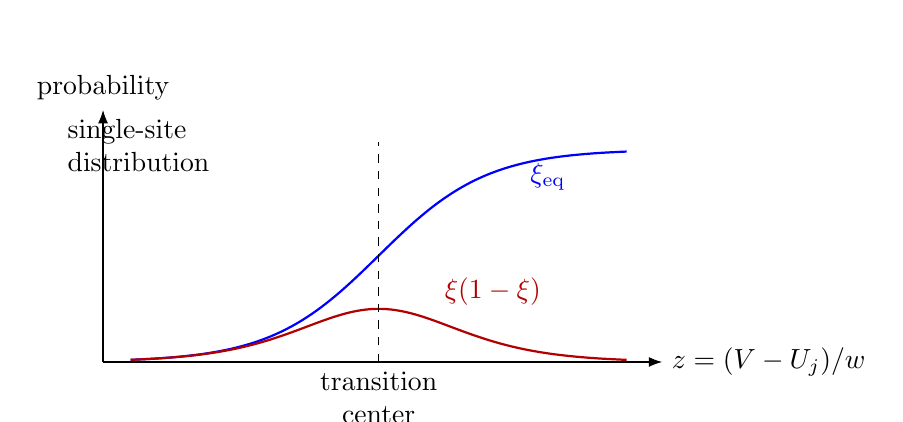
\begin{tikzpicture}[x=1cm,y=1cm,>=Latex]
  \draw[->] (0,0) -- (7.1,0) node[right] {$z=(V-U_j)/w$};
  \draw[->] (0,0) -- (0,3.2) node[above] {probability};
  \draw[thick,blue,domain=0.35:6.65,samples=100]
    plot(\x,{2.7/(1+exp(-1.45*(\x-3.5)))});
  \draw[thick,red!70!black,domain=0.35:6.65,samples=100]
    plot(\x,{2.7*exp(-1.45*(\x-3.5))/(1+exp(-1.45*(\x-3.5)))^2});
  \draw[dashed] (3.5,0) -- (3.5,2.8);
  \node[blue] at (5.65,2.35) {$\xi_{\eq}$};
  \node[red!70!black] at (4.95,0.9) {$\xi(1-\xi)$};
  \node[align=center] at (3.5,-0.45) {transition\\center};
  \node[align=left] at (0.45,2.75) {single-site\\distribution};
\end{tikzpicture}
\caption{Two-state occupation gives the Ch1 logistic. The local weight in
$\dd Q/\dd V$ is proportional to $\xi(1-\xi)/w$.}
\label{fig:logistic_distribution}
\end{figure}

\subsection{다자리 평균장과 Bragg--Williams 자유에너지}
한 전이가 많은 동등한 자리를 가진다면, 조성 $\theta$ 의 molar free energy 를
Bragg--Williams 평균장으로 쓸 수 있다 \cite{huggins1941,bazant2013,newman}:
\begin{equation}
g(\theta,T)=g^0+\Delta g^0\,\theta
  +RT\{\theta\ln\theta+(1-\theta)\ln(1-\theta)\}
  +\Omega\,\theta(1-\theta).
\label{eq:bragg_williams}
\end{equation}
세 항의 역할은 분명하다. $\Delta g^0$ 는 중심 전위 또는 표준 반응 자유에너지, 로그 항은
무작위 점유 분포의 configurational free energy, $\Omega$ 는 평균장 상호작용이다. $\Omega>0$ 이면
서로 다른 점유 상태가 섞이는 것을 벌하고, $\Omega\rightarrow2RT$ 에 가까워질수록 중심 기울기가
작아져 plateau 와 상분리 임계에 접근한다.

식~\eqref{eq:bragg_williams} 를 미분하면 de-lithiation progress 의 평형 전위는, 상수항을 $U^0$ 에
흡수했을 때,
\begin{equation}
U(\xi,T)
=U^0(T)+\frac{RT}{F}\ln\frac{\xi}{1-\xi}
  +\frac{\Omega}{F}(1-2\xi)
\label{eq:regular_solution_ocv}
\end{equation}
로 쓸 수 있다. 여기서 로그항의 온도 미분이 바로 식~\eqref{eq:sign_config_intro} 의 configurational
엔트로피 계수다.

% ====================================================================
\section{점유 분포에서 configurational entropy 까지}
\label{sec:config_entropy}
% ====================================================================
\subsection{Shannon--Boltzmann 형태}
단일 자리에서 가능한 두 상태의 확률은 $(1-\theta,\theta)$ 이다. 확률 분포의 entropy 는
\begin{equation}
S_{\config}
  =-R\sum_i p_i\ln p_i
  =-R\{(1-\theta)\ln(1-\theta)+\theta\ln\theta\}
\label{eq:sconfig}
\end{equation}
이다. 이 식은 단순 암기가 아니라 조합수에서 직접 나온다. $N$ 개 자리 중 $N\theta$ 개를 점유시키는
미시상태 수는
\begin{equation}
W=\frac{N!}{(N\theta)![N(1-\theta)]!}.
\label{eq:multiplicity}
\end{equation}
Stirling 근사 $\ln N!\simeq N\ln N-N$ 을 넣으면
\begin{equation}
\frac{k_{\mathrm B}\ln W}{N}
  =-k_{\mathrm B}\{\theta\ln\theta+(1-\theta)\ln(1-\theta)\},
\label{eq:stirling_s}
\end{equation}
이고 1 mol 자리 기준으로 $k_{\mathrm B}N_A=R$ 를 곱하면 식~\eqref{eq:sconfig} 이다.

\subsection{부분몰 항과 전위 온도계수}
식~\eqref{eq:sconfig} 의 $\theta$ 미분은
\begin{equation}
\frac{\partial S_{\config}}{\partial\theta}
  =-R\ln\frac{\theta}{1-\theta}.
\label{eq:partial_s_lith}
\end{equation}
이는 lithiation coordinate 로 쓴 부분몰 configurational entropy 이다. 본 장은 $\xi$ 를
de-lithiation progress 로 쓰므로 $\theta=1-\xi$ 로 바꾸면
\begin{equation}
\Delta S_{\config}^{(\mathrm{delith})}
=R\ln\frac{\xi}{1-\xi}.
\label{eq:partial_s_delith}
\end{equation}
따라서 한 전이 내부에서
\begin{equation}
\left.\frac{\partial U_j}{\partial T}\right|_{\xi}
  =\frac{\Delta S_{\rxn,j}^0}{F}
  +\frac{R}{F}\ln\frac{\xi}{1-\xi}
  +\left.\frac{\partial U_j}{\partial T}\right|_{\vib+\el,\mathrm{residual}},
\label{eq:single_peak_dudt}
\end{equation}
이다. $\xi=1/2$ 에서는 로그항이 0 이므로 $\Delta S_{\rxn,j}^0$ 는 전이 중심 표준값이다.

\begin{warnbox}
\textbf{이중계산 B.} $\Delta S_{\rxn,j}^0$ 를 전이 폭 전체의 조성 의존 entropy 함수로 해석하면 안 된다.
그 값은 $\xi=1/2$ 중심의 표준 반응 entropy 이고, 봉우리 내부에서 급격히 변하는 configurational
항은 logistic 폭 $w=RT/F$ 가 이미 만든다. 따라서
``$\Delta S_{\rxn,j}^0$ + 별도 $S_{\config}$'' 를 쓸 때 별도 항은 중심에서 0 인 식~\eqref{eq:partial_s_delith}
이어야 하며, 중심값에 같은 mixing entropy 를 다시 넣지 않는다.
\end{warnbox}

\begin{figure}[t]
\centering
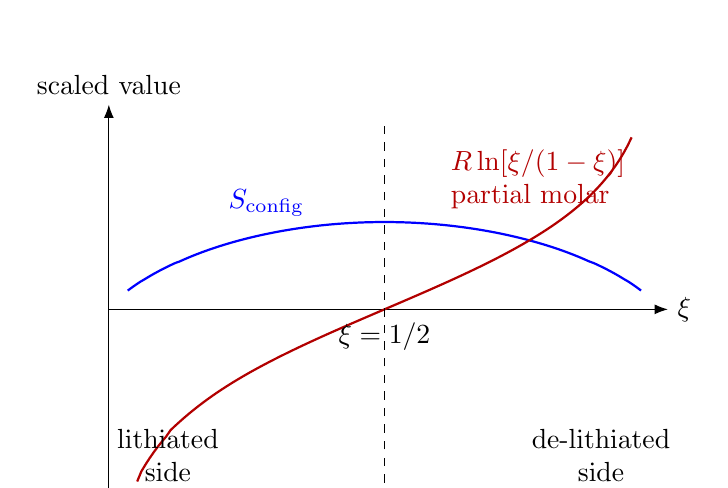
\begin{tikzpicture}[x=1cm,y=1cm,>=Latex]
  \draw[->] (0,0) -- (7.1,0) node[right] {$\xi$};
  \draw[->] (0,-2.4) -- (0,2.6) node[above] {scaled value};
  \draw[thick,blue,domain=0.24:6.76,samples=120]
    plot(\x,{1.6*(-((\x/7)*ln(\x/7)+(1-\x/7)*ln(1-\x/7)))});
  \draw[thick,red!70!black,domain=0.36:6.64,samples=120]
    plot(\x,{0.75*ln((\x/7)/(1-\x/7))});
  \draw[dashed] (3.5,-2.2) -- (3.5,2.4);
  \node[blue] at (2.0,1.35) {$S_{\config}$};
  \node[red!70!black,align=left] at (5.45,1.65) {$R\ln[\xi/(1-\xi)]$\\partial molar};
  \node at (3.5,-0.35) {$\xi=1/2$};
  \node[align=center] at (0.75,-1.85) {lithiated\\side};
  \node[align=center] at (6.25,-1.85) {de-lithiated\\side};
\end{tikzpicture}
\caption{Configurational entropy is maximal at half occupation, but its partial
molar contribution changes sign and diverges at the ends.}
\label{fig:sconfig}
\end{figure}

% ====================================================================
\section{세 분포 기반 entropy decomposition}
\label{sec:entropy_decomp}
% ====================================================================
하프셀에서 측정하는 $\partial U/\partial T$ 는 단일 종류의 entropy 가 아니다. 이 장에서는 다음 세
분포를 분리해 둔다.
\begin{equation}
\Delta S(x,T)=\Delta S_{\config}(x,T)+\Delta S_{\vib}(x,T)+\Delta S_{\el}(x,T),
\qquad
\frac{\partial U_\oc}{\partial T}=\frac{\Delta S}{F}.
\label{eq:three_entropy}
\end{equation}

\subsection{Configurational: 격자기체 분포}
Configurational 항은 앞 절의 점유 분포에서 나온다. 한 전이 중심 근방에서는
\begin{equation}
\Delta S_{\config,j}(\xi_j)=R\ln\frac{\xi_j}{1-\xi_j}.
\label{eq:config_j}
\end{equation}
여러 전이가 겹치면 이 항은 각 전이의 local differential-capacity weight 로 평균된다
(\S\ref{sec:overlap}). 이 항은 저 Li 또는 말단 조성에서 큰 양/음 신호를 만들 수 있지만, 실제 데이터에서는
전이 폭, 상호작용, staging end point, 측정 cut-off 때문에 수학적 무한대가 잘려 보인다.

\subsection{Vibrational: phonon Bose--Einstein 분포}
격자 진동의 미시상태는 phonon occupation 이다. 모드 $k$ 의 Bose--Einstein 평균 점유수는
\begin{equation}
n_k=\frac{1}{\exp(\beta\hbar\omega_k)-1},
\label{eq:be}
\end{equation}
이고, harmonic phonon entropy 는
\begin{equation}
S_{\vib}
=R\sum_k\{(1+n_k)\ln(1+n_k)-n_k\ln n_k\}.
\label{eq:svib}
\end{equation}
Li 삽입 또는 탈리튬화는 결합 강성, 층간 거리, phonon density of states 를 바꾸므로
$\Delta S_{\vib}$ 를 만든다. 흑연에서는 고 lithiation 쪽의 음의 baseline 이 vibrational 기여로 해석되는
경우가 많다 \cite{reynier2003,allart2018,jpcc2021}. 실용 피팅에서는 한 전이 폭 안에서
$\Delta S_{\vib}$ 가 천천히 변한다고 보고 중심 표준값 $\Delta S_{\rxn,j}^0$ 에 흡수한다.

\subsection{Electronic: Fermi--Dirac 분포와 Sommerfeld 항}
전자 entropy 는 Fermi--Dirac 분포
\begin{equation}
f(E)=\frac{1}{\exp[(E-E_F)/k_{\mathrm B}T]+1}
\label{eq:fd}
\end{equation}
에서 나온다. 금속 또는 좁은 gap 상태에서 저온 Sommerfeld 전개는
\begin{equation}
S_{\el}=\frac{\pi^2}{3}k_{\mathrm B}^2T\,g(E_F)
\label{eq:sommerfeld}
\end{equation}
를 준다. 여기서 $g(E_F)$ 는 Fermi level 의 density of states 이다. Ch1 v9 의 electronic 항은 이
Fermi--Dirac entropy 를 하프셀 entropy coefficient 에 넣는 확장이다. 흑연 음극에서는 보통 작은 항으로
취급하지만, LCO 같은 metal--insulator transition 게이트에서는 $\Delta S_{\el}$ 가 눈에 띄게 변할 수 있다.
삽입 기준 $\Delta S_e<0$ 로 두면, 본 장의 de-lithiation coordinate 에서는 부호 변환을 명시해야 한다.

\begin{keybox}
전이별 상수 $\Delta S_{\rxn,j}^0$ 는 configurational 중심값 0 에서 남는 표준값이다. 실제 내용은
vibrational baseline, electronic 중심값, 그리고 전이 표준 반응 entropy 를 포함한다. 봉우리 내부의
비선형성은 $\Delta S_{\rxn,j}^0(x)$ 를 임의 함수로 만들지 않아도, 겹침 가중과 configurational 로그항에서
자동으로 생긴다.
\end{keybox}

% ====================================================================
\section{겹친 전이의 entropy coefficient: local dQ/dV weight}
\label{sec:overlap}
% ====================================================================
\subsection{음함수 미분}
여러 staging 전이가 같은 전압 범위에서 겹치면 관측 $U_\oc(x,T)$ 는 각 전이의 계단을 단순히 이어 붙인
함수가 아니다. 평형 조건은
\begin{equation}
x=\frac{1}{Q_{\mathrm{tot}}}\sum_j Q_j\,\xi_j(U_\oc,T),
\label{eq:implicit_x}
\end{equation}
이다. 같은 $x$ 에서 온도를 바꾸며 미분하면
\begin{equation}
0=\sum_j Q_j\left[
\left.\frac{\partial \xi_j}{\partial U}\right|_T
\left.\frac{\partial U_\oc}{\partial T}\right|_x
+\left.\frac{\partial \xi_j}{\partial T}\right|_U
\right],
\label{eq:implicit_diff}
\end{equation}
따라서
\begin{equation}
\left.\frac{\partial U_\oc}{\partial T}\right|_x
=-\frac{\sum_j Q_j\,\left.\partial \xi_j/\partial T\right|_U}
        {\sum_j Q_j\,\left.\partial \xi_j/\partial U\right|_T}.
\label{eq:dudt_implicit}
\end{equation}
logistic 전이에서
\begin{equation}
g_j=\left.\frac{\partial \xi_j}{\partial U}\right|_T
=\frac{\xi_j(1-\xi_j)}{w_j}
\label{eq:gj}
\end{equation}
는 local $\dd Q/\dd V$ 봉우리 모양이다. 중심 표준값만 남기면
\begin{equation}
\boxed{\;
\left.\frac{\partial U_\oc}{\partial T}\right|_x
=\frac{1}{F}\,
\frac{\sum_j Q_j\,g_j(x)\,\Delta S_{\rxn,j}^0}
     {\sum_j Q_j\,g_j(x)}
\;}
\label{eq:overlap_simple}
\end{equation}
이다. 즉 관측 entropy coefficient 는 전이별 $\Delta S_{\rxn,j}^0/F$ 의 계단이 아니라,
local differential-capacity weight $Q_jg_j/\sum_kQ_kg_k$ 로 평균된 연속 함수다.

\subsection{완전식: overlap weight 와 봉우리 내부 config 를 함께}
식~\eqref{eq:overlap_simple} 은 중심 표준 entropy 의 겹침만 보이는 식이다. logistic 폭의 온도 의존까지
완전히 포함하면 각 전이의 위치 변수
\begin{equation}
z_j=\ln\frac{\xi_j}{1-\xi_j}
\label{eq:zj}
\end{equation}
가 configurational 항을 만든다. de-lithiation progress 규약에서
\begin{equation}
\boxed{\;
\left.\frac{\partial U_\oc}{\partial T}\right|_x
=\frac{1}{F}\,
\frac{\sum_j Q_jg_j\{\Delta S_{\rxn,j}^0+Rz_j\}}
     {\sum_j Q_jg_j}
\;}
\label{eq:overlap_full}
\end{equation}
가 관측 entropy coefficient 의 실용식이다. 수치 검증에서는 다온도 유한차분으로 얻은
$\partial U_\oc/\partial T$ 와 식~\eqref{eq:overlap_full} 이 부동소수점 수준에서 일치했고, 중심값만
사용한 식~\eqref{eq:overlap_simple} 의 오차는 누락한 configurational 항의 크기와 같았다.

\begin{figure}[t]
\centering
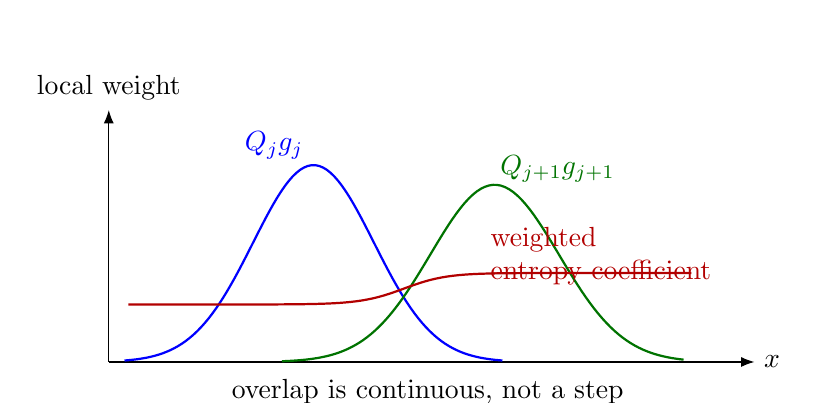
\begin{tikzpicture}[x=1cm,y=1cm,>=Latex]
  \draw[->] (0,0) -- (8.2,0) node[right] {$x$};
  \draw[->] (0,0) -- (0,3.2) node[above] {local weight};
  \draw[thick,blue,domain=0.2:5.0,samples=100]
    plot(\x,{2.5*exp(-0.85*(\x-2.6)*(\x-2.6))});
  \draw[thick,green!45!black,domain=2.2:7.3,samples=100]
    plot(\x,{2.25*exp(-0.75*(\x-4.9)*(\x-4.9))});
  \draw[thick,red!70!black,domain=0.25:7.4,samples=100]
    plot(\x,{(0.28*2.5*exp(-0.85*(\x-2.6)*(\x-2.6))
      +0.68*2.25*exp(-0.75*(\x-4.9)*(\x-4.9)))/
      (2.5*exp(-0.85*(\x-2.6)*(\x-2.6))
      +2.25*exp(-0.75*(\x-4.9)*(\x-4.9)))+0.45});
  \node[blue] at (2.1,2.75) {$Q_jg_j$};
  \node[green!45!black] at (5.7,2.45) {$Q_{j+1}g_{j+1}$};
  \node[red!70!black,align=left] at (6.25,1.35) {weighted\\entropy coefficient};
  \node at (4.05,-0.38) {overlap is continuous, not a step};
\end{tikzpicture}
\caption{When two dQ/dV peaks overlap, $\partial U/\partial T$ is a local
weighted average. The transition between entropy coefficients is continuous.}
\label{fig:overlap_weight}
\end{figure}

\begin{procedurebox}
하프셀 데이터에서 식~\eqref{eq:overlap_full} 을 쓰는 절차는 다음이다.
(1) 충분히 낮은 rate 의 다온도 $\dd Q/\dd V$ 를 얻는다.
(2) Ch1 logistic 전이 모델로 $Q_j,U_j(T),w_j(T)$ 를 동시에 맞춘다.
(3) 중심 기울기 $\dd U_j/\dd T$ 에서 $\Delta S_{\rxn,j}^0=F\,\dd U_j/\dd T$ 를 얻는다.
(4) 각 $x$ 에서 $\xi_j,g_j,z_j$ 를 계산한다.
(5) 식~\eqref{eq:overlap_full} 로 $\partial U_\oc/\partial T$ 를 산출하고,
식~\eqref{eq:qrev_intro} 로 $\dot Q_\rev$ 를 계산한다.
\end{procedurebox}

% ====================================================================
\section{상호작용과 유효 폭: $w_{\eff}(\Omega)$}
\label{sec:weff}
% ====================================================================
정규용액 항 $\Omega\xi(1-\xi)$ 는 logistic 봉우리의 폭을 바꾼다. 식~\eqref{eq:regular_solution_ocv} 의
기울기는
\begin{equation}
\frac{\dd U}{\dd \xi}
=\frac{RT}{F}\left[\frac{1}{\xi(1-\xi)}-\frac{2\Omega}{RT}\right].
\label{eq:regular_slope}
\end{equation}
중심 $\xi=1/2$ 에서는
\begin{equation}
\left.\frac{\dd U}{\dd \xi}\right|_{\xi=1/2}
=\frac{4RT-2\Omega}{F}.
\label{eq:center_slope}
\end{equation}
상호작용 없는 logistic 의 중심 기울기와 정합시키면
\begin{equation}
\boxed{\;
w_{\eff}(\Omega)=\frac{w}{1-\Omega/(2RT)},\qquad w=\frac{RT}{F},\quad \Omega<2RT.
\;}
\label{eq:weff}
\end{equation}
$\Omega\rightarrow2RT^{-}$ 에서 $w_{\eff}$ 는 발산한다. 물리적으로는 단순히 봉우리가 무한히 넓어진다는
뜻이 아니라, 평균장 spinodal/plateau 한계에 접근한다는 뜻이다. 그 근방에서는 균일 조성 모델이
상분리 domain, nucleation barrier, hysteresis 를 평균낸 표현에 불과하다.

\begin{figure}[t]
\centering
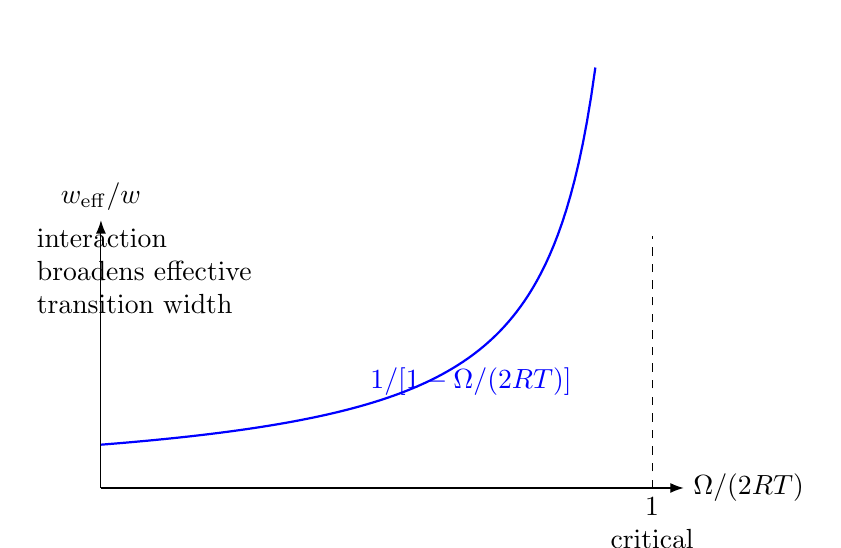
\begin{tikzpicture}[x=1cm,y=1cm,>=Latex]
  \draw[->] (0,0) -- (7.4,0) node[right] {$\Omega/(2RT)$};
  \draw[->] (0,0) -- (0,3.4) node[above] {$w_{\eff}/w$};
  \draw[thick,blue,domain=0:6.28,samples=120]
    plot(\x,{0.55/(1-\x/7)});
  \draw[dashed] (7,0) -- (7,3.2);
  \node[align=center] at (7,-0.45) {$1$\\critical};
  \node[blue] at (4.7,1.35) {$1/[1-\Omega/(2RT)]$};
  \node[align=left] at (0.55,2.75) {interaction\\broadens effective\\transition width};
\end{tikzpicture}
\caption{Mean-field interaction changes the apparent transition width. The
formula is a center-slope match valid below the critical limit.}
\label{fig:weff}
\end{figure}

온도 미분에서 $\Omega$ 자체가 약하게 $T$ 의존하면 $\partial w_{\eff}/\partial T$ 가 추가 항을 만든다.
이 장에서는 이 효과를 2차 보정으로 둔다. 실제 coin half-cell 피팅에서 $\Omega(T)$ 를 둘 만큼 데이터가
충분하지 않다면, 먼저 $w_{\eff}$ 를 전이 폭 parameter 로 맞추고 $\Delta S_{\rxn,j}^0$ 와 config 항의
이중계산 여부를 점검하는 편이 더 견고하다.

% ====================================================================
\section{히스테리시스: 가역 평균과 비가역 gap 의 분리}
\label{sec:hysteresis}
% ====================================================================
흑연 OCV 는 충방전 branch 가 완전히 겹치지 않는다. 그러나 branch gap 을 가역 entropy 로 넣으면
비가역 소산을 섞게 된다. 각 branch $d\in\{\ch,\dis\}$ 의 중심 전위를
\begin{equation}
U_j^{(d)}=U_j^{\rev}\pm\frac{1}{2}\Delta U_j^{\hys}
\label{eq:hys_center}
\end{equation}
로 두고, branch 별 봉우리 $g_j^{(d)}$ 를 계산하면
\begin{equation}
\left.\frac{\partial U_\oc^{(d)}}{\partial T}\right|_x
=\frac{1}{F}
\frac{\sum_j Q_jg_j^{(d)}\{\Delta S_{\rxn,j}^{0,(d)}+Rz_j^{(d)}\}}
     {\sum_j Q_jg_j^{(d)}}.
\label{eq:hys_branch}
\end{equation}
열역학적 가역 평균은
\begin{equation}
\left.\frac{\partial U^{\rev}}{\partial T}\right|_x
=\frac{1}{2}\left(
\left.\frac{\partial U^{\ch}}{\partial T}\right|_x+
\left.\frac{\partial U^{\dis}}{\partial T}\right|_x
\right)
\label{eq:hys_average}
\end{equation}
로 정의한다. 반면 $\Delta U^\hys$ 자체에 전류가 지나며 생기는 열은
\begin{equation}
\dot Q_{\hys,\irr}\simeq I\,\Delta U^\hys
\label{eq:hys_heat}
\end{equation}
꼴의 비가역열이다. 온도에 따라 hysteresis gap 이 달라질 수는 있지만, 그 효과는
$\partial U^\rev/\partial T$ 로 표현되는 reversible heat 와 별도 budget 으로 분리한다.

\begin{warnbox}
이 장은 coin half-cell 의 단일 전극 entropy coefficient 를 다룬다. 충전 branch 와 방전 branch 를 평균해
가역 부분을 정의할 수는 있지만, 이를 full-cell 열수지로 합성하거나 cathode 신호와 결합하지 않는다.
\end{warnbox}

% ====================================================================
\section{극한과 corner checks}
\label{sec:limits}
% ====================================================================
식이 맞는지 보려면 극한에서 어떤 값을 주는지 확인해야 한다.

\begin{longtable}{p{0.23\linewidth}p{0.38\linewidth}p{0.30\linewidth}}
\caption{Ch2 v4-07 limit checks for the half-cell entropy coefficient.}
\label{tab:limits}\\
\toprule
극한 & 거동 & 해석 \\
\midrule
\endfirsthead
\toprule
극한 & 거동 & 해석 \\
\midrule
\endhead
$\xi\rightarrow0$ &
$R\ln[\xi/(1-\xi)]\rightarrow-\infty$ &
de-lithiation coordinate 에서 lithiated end 의 부분몰 configurational 항이 음으로 발산한다. \\
$\xi\rightarrow1$ &
$R\ln[\xi/(1-\xi)]\rightarrow+\infty$ &
de-lithiated end 에서 양으로 발산한다. 실제 전극에서는 end-member cut-off 와 상분리가 이를 자른다. \\
$\xi=1/2$ &
$R\ln[\xi/(1-\xi)]=0$ &
$\partial U/\partial T=\Delta S_{\rxn,j}^0/F$; 표준 중심값 회수. \\
$\Omega\rightarrow2RT^{-}$ &
$w_{\eff}\rightarrow\infty$ &
평균장 임계/plateau 접근. 균일 logistic 해석의 적용 한계. \\
단일 봉우리 &
식~\eqref{eq:overlap_full} 이 $\{\Delta S_j^0+Rz_j\}/F$ 로 환원 &
겹침이 없는 경우에도 config 항은 남는다. \\
고온 electronic &
$S_{\el}\propto T\,g(E_F)$ 항이 커질 수 있음 &
metallic 또는 MIT 근방 전극에서는 $\Delta S_{\el}$ 의 조성 의존을 상수로 묶으면 안 된다. \\
\bottomrule
\end{longtable}

이 표는 ``$\Delta S_{\rxn,j}$ 를 전이별 상수로 둘 수 있는가''라는 실무 질문의 답을 준다.
상수 근사는 \textbf{중심 표준값}에 대해서만 타당하다. 봉우리 내부의 급격한 변화는
configurational 분포 항이 담당하고, 인접 봉우리 사이의 매끄러운 변화는 겹침 가중이 담당한다.
따라서 측정 $\partial U/\partial T(x)$ 가 비선형이라고 해서 곧바로 $\Delta S_{\rxn,j}^0$ 를 임의의
$x$ 함수로 만들 필요는 없다. 다만 vibrational 또는 electronic 항이 같은 전이 폭 안에서 급변하는
경우, 예를 들어 LCO 의 MIT gate 처럼 $g(E_F)$ 가 급변하는 경우에는 그 항만 별도의 $x$ 의존으로 둔다.

% ====================================================================
\section{가역 발열: entropy coefficient 에서 heat rate 로}
\label{sec:reversible_heat}
% ====================================================================
Bernardi--Newman 에너지 수지에서 단일 전극 하프셀의 reversible heat 항은
\begin{equation}
\boxed{\;\dot Q_\rev=-I\,T\,\left.\frac{\partial U_\oc}{\partial T}\right|_x
=-\frac{I\,T}{F}\Delta S(x)\;}
\label{eq:qrev_final}
\end{equation}
이다 \cite{bernardi1985,newman}. 이 부호는 본 장에서 고정한다. $I>0$ 방전이고
$\partial U/\partial T>0$ 이면 $\dot Q_\rev<0$ 이므로 방전 가역항은 흡열이다.
충전에서는 $I<0$ 이 되어 같은 entropy coefficient 가 반대 부호의 가역열을 낸다.

식~\eqref{eq:overlap_full} 을 넣으면 coin half-cell 의 실용 reversible heat 는
\begin{equation}
\dot Q_\rev(x,T)
=-\frac{I\,T}{F}
\frac{\sum_j Q_jg_j(x,T)\{\Delta S_{\rxn,j}^0+Rz_j(x,T)
 +\Delta S_{\vib,j}^{\mathrm{res}}+\Delta S_{\el,j}^{\mathrm{res}}\}}
     {\sum_j Q_jg_j(x,T)}.
\label{eq:qrev_overlap}
\end{equation}
여기서 $\Delta S_{\vib,j}^{\mathrm{res}}$ 와 $\Delta S_{\el,j}^{\mathrm{res}}$ 는 중심 표준값에 이미
흡수하지 않은 residual 조성 의존만 뜻한다. 기본 흑연 half-cell 해석에서는 이 residual 을 0 으로 두고,
$\Delta S_{\rxn,j}^0$ 와 configurational 로그항, overlap weight 부터 검증한다.

\subsection{다온도 dQ/dV workflow}
v3 skeleton 이 강조한 다온도 $\dd Q/\dd V$ 경로는 이 통계열역학식으로 더 명확해진다.
\begin{enumerate}[leftmargin=1.7em,itemsep=2pt]
\item 각 온도 $T_k$ 에서 quasi-equilibrium coin half-cell $\dd Q/\dd V$ 를 측정한다.
\item 같은 $Q_j$ 구조를 공유하되 $U_j(T_k)$ 와 필요한 폭 parameter 를 허용해 Ch1 logistic/MSMR 꼴을
동시 피팅한다.
\item $U_j(T)$ 를 저차 함수로 회귀하고 중심 entropy coefficient
$\partial U_j/\partial T=\Delta S_{\rxn,j}^0/F$ 를 얻는다.
\item 각 $x$ 에서 $\xi_j,g_j,z_j$ 를 계산해 식~\eqref{eq:overlap_full} 의
$\partial U_\oc/\partial T$ 를 얻는다.
\item 식~\eqref{eq:qrev_final} 로 reversible heat 를 계산한다. Hysteresis gap 과 rate overpotential 은
비가역열 budget 으로 분리한다.
\end{enumerate}

\begin{srcbox}
Bernardi 등은 전지 에너지 수지를 가역항과 비가역항으로 분해했다 \cite{bernardi1985}. Newman 의
전기화학 열역학은 $U(T)$ 기울기와 reaction entropy 의 관계를 닫는다 \cite{newman}. 흑연 entropy
profile 은 Reynier--Yazami--Fultz 및 Allart 등의 potentiometric 분석과 정합한다
\cite{reynier2003,allart2018}. MSMR 온도 의존 분석은 전이별 $U_j(T)$ 회귀의 template 를 준다
\cite{msmr_partI,msmr_partII}. 본 장의 추가점은 이 체인을 점유 분포, configurational 로그항,
overlap weight 로 명시적으로 연결한 것이다.
\end{srcbox}

% ====================================================================
\section{정직한 적용 범위와 남는 불확실성}
\label{sec:scope}
% ====================================================================
확정된 범위는 다음과 같다. 첫째, 단일 전극 coin half-cell 의 $\partial U/\partial T$ 와
reversible heat 만 다룬다. 둘째, $\xi$ 는 de-lithiation progress 이고, 이에 따라 config 항의 부호는
$+R\ln[\xi/(1-\xi)]$ 이다. 셋째, $\Delta S_{\rxn,j}^0$ 는 중심 표준값이며, 분포가 만드는 config 항과
이중계산하지 않는다. 넷째, hysteresis branch 의 평균은 reversible entropy coefficient 로 쓰되,
branch gap 자체는 irreversible heat 로 분리한다.

남는 불확실성은 하나로 압축된다. Electrochimica Acta 2019 occupation-transition prototype 은
$\dd Q/\dd V$ 와 entropy profiling 을 결합한 가까운 선례지만, 현재 장에서는 full text 식을 직접 확보하지
못한 상태라 방법 수준 인용으로만 둔다. 따라서 실제 실험 데이터에 적용할 때는 그 논문의 상세 model 식을
원문으로 대조한 뒤 본 장의 식~\eqref{eq:overlap_full} 과 같은지, 또는 dilute-limit 보정이 필요한지
확인해야 한다.

% ====================================================================
\section*{맺음}
\addcontentsline{toc}{section}{맺음}
% ====================================================================
Chapter 2 v4-07 의 결론은 짧다. Ch1 의 logistic 봉우리는 통계 분포다. 그 분포의 폭 $RT/F$ 는
configurational entropy 를 만들고, 전이 중심의 $\Delta S_{\rxn,j}^0$ 는 vibrational/electronic 중심값을
포함한 표준 reaction entropy 로 남는다. 여러 봉우리가 겹치면 $\partial U/\partial T$ 는 local
$\dd Q/\dd V$ weight 로 연속 평균되고, hysteresis 는 reversible average 와 irreversible gap 으로 분리된다.
이렇게 얻은 entropy coefficient 를 Bernardi 식에 넣으면 coin half-cell reversible heat 가 닫힌다:
$\dot Q_\rev=-IT\,\partial U/\partial T$.

% ====================================================================
\begin{thebibliography}{99}
\bibitem{bernardi1985}
D. Bernardi, E. Pawlikowski, J. Newman,
``A General Energy Balance for Battery Systems,''
\emph{J. Electrochem. Soc.} \textbf{132}(1), 5--12 (1985).
DOI: 10.1149/1.2113792.

\bibitem{newman}
J. Newman, K. E. Thomas-Alyea,
\emph{Electrochemical Systems}, 3rd ed., Wiley (2004).
Tier: textbook basis for electrochemical thermodynamics and entropy coefficients.

\bibitem{reynier2003}
Y. Reynier, R. Yazami, B. Fultz,
``The entropy and enthalpy of lithium intercalation into graphite,''
\emph{J. Power Sources} \textbf{119--121}, 850--855 (2003).
DOI: 10.1016/S0378-7753(03)00285-4.

\bibitem{allart2018}
D. Allart \emph{et al.},
``Model of Lithium Intercalation into Graphite by Potentiometric Analysis with
Equilibrium and Entropy Change Curves of the Graphite Electrode,''
\emph{J. Electrochem. Soc.} \textbf{165}(2), A380 (2018).
DOI: 10.1149/2.1251802jes.

\bibitem{occupation2019}
``Transitions of lithium occupation in graphite: A physically informed model in the dilute
lithium occupation limit supported by electrochemical and thermodynamic measurements,''
\emph{Electrochimica Acta} (2019).
DOI: 10.1016/j.electacta.2019.135634.
Tier: method-level citation; full-text equations not re-derived here.

\bibitem{chemmater2015}
``Intercalation Compounds from LiH and Graphite: Relative Stability of Metastable Stages\ldots,''
\emph{Chem. Mater.} \textbf{27} (2015).
DOI: 10.1021/acs.chemmater.5b00235.
Tier: abstract-level formation enthalpy context.

\bibitem{jpcc2021}
``Thermodynamic Analysis of Li-Intercalated Graphite by First-Principles with
Vibrational and Configurational Contributions,''
\emph{J. Phys. Chem. C} \textbf{125} (2021).
DOI: 10.1021/acs.jpcc.1c08992.
Tier: abstract-level support for vib/config contributions.

\bibitem{msmr_partI}
``Quantifying the Entropy and Enthalpy of Insertion Materials for Battery Applications
Via the Multi-Species, Multi-Reaction Model,''
\emph{J. Electrochem. Soc.} (2024).
DOI: 10.1149/1945-7111/ad1d27.

\bibitem{msmr_partII}
``Quantifying the Temperature Dependence of the MSMR Model Part II: Estimation of
Entropy Coefficient for Meso-Carbon Micro-Bead Graphite,''
\emph{J. Electrochem. Soc.} (2024).
DOI: 10.1149/1945-7111/ad70d9.

\bibitem{standardised2024}
``A Standardised Potentiometric Method for the Effective Parameterisation of
Reversible Heating in a Lithium-Ion Cell,''
\emph{J. Electrochem. Soc.} (2024).
DOI: 10.1149/1945-7111/ad4918.

\bibitem{hysteresis2018}
``Uncertainties in entropy due to temperature path dependent voltage hysteresis in
Li-ion cells,''
\emph{J. Power Sources} (2018).
DOI: 10.1016/j.jpowsour.2018.05.060.

\bibitem{huggins1941}
M. L. Huggins,
``Solutions of Long Chain Compounds,''
\emph{J. Chem. Phys.} \textbf{9}, 440 (1941).
DOI: 10.1063/1.1750930.

\bibitem{bazant2013}
M. Z. Bazant,
``Theory of Chemical Kinetics and Charge Transfer based on Nonequilibrium Thermodynamics,''
\emph{Accounts of Chemical Research} \textbf{46}(5), 1144--1160 (2013).
DOI: 10.1021/ar300145c.
\end{thebibliography}

\end{document}
